\documentclass[a4paper,10pt,justified,openany]{tufte-book}
\usepackage[utf8]{inputenc}
\usepackage{graphicx}
\hypersetup{colorlinks} % Comment this line if you don't wish to have colored links

\usepackage{microtype} % Improves character and word spacing

\usepackage{lipsum} % Inserts dummy text

\usepackage{booktabs} % Better horizontal rules in tables

\usepackage{amssymb}

\usepackage{graphicx} % Needed to insert images into the document
\graphicspath{{graphics/}} % Sets the default location of pictures
\setkeys{Gin}{width=\linewidth,totalheight=\textheight,keepaspectratio} % Improves figure scaling

\usepackage{fancyvrb} % Allows customization of verbatim environments
\fvset{fontsize=\normalsize} % The font size of all verbatim text can be changed here

\newcommand{\hangp}[1]{\makebox[0pt][r]{(}#1\makebox[0pt][l]{)}} % New command to create parentheses around text in tables which take up no horizontal space - this improves column spacing
\newcommand{\hangstar}{\makebox[0pt][l]{*}} % New command to create asterisks in tables which take up no horizontal space - this improves column spacing

\usepackage{xspace} % Used for printing a trailing space better than using a tilde (~) using the \xspace command

\newcommand{\monthyear}{\ifcase\month\or January\or February\or March\or April\or May\or June\or July\or August\or September\or October\or November\or December\fi\space\number\year} % A command to print the current month and year

\newcommand{\openepigraph}[2]{ % This block sets up a command for printing an epigraph with 2 arguments - the quote and the author
\begin{fullwidth}
\sffamily\large
\begin{doublespace}
\noindent\allcaps{#1}\\ % The quote
\noindent\allcaps{#2} % The author
\end{doublespace}
\end{fullwidth}
}

\newcommand{\blankpage}{\newpage\hbox{}\thispagestyle{empty}\newpage} % Command to insert a blank page



\usepackage{makeidx} % Used to generate the index
\makeindex % Generate the index which is printed at the end of the document

\usepackage{listings}
\usepackage[toc,page]{appendix}
% Title Page
\title{Manuel d'utilisation de RoCaWeb (V3)}
\author{Team RoCaWeb}

\begin{document}



\frontmatter


%----------------------------------------------------------------------------------------

\maketitle % Print the title page

%----------------------------------------------------------------------------------------
%	COPYRIGHT PAGE
%----------------------------------------------------------------------------------------

\newpage
\begin{fullwidth}
~\vfill
\thispagestyle{empty}
\setlength{\parindent}{0pt}
\setlength{\parskip}{\baselineskip}
Copyright \copyright\ \the\year\ \thanklessauthor

\par\smallcaps{Published by T\'elecom-Bretagne et Kereval}

%\par\smallcaps{\url{http://www.bookwebsite.com}}

%\par License information.\index{license}

\par\textit{First printing, \monthyear}
\end{fullwidth}

%----------------------------------------------------------------------------------------

\tableofcontents % Print the table of contents

%----------------------------------------------------------------------------------------


%----------------------------------------------------------------------------------------
%	DEDICATION PAGE
%----------------------------------------------------------------------------------------



%\begin{abstract}

%\end{abstract}


\chapter{Introduction}
\section{Introduction}
Dans ce petit guide, nous allons expliquer le fonctionnement de la version courante de Rocaweb. Nous informons dès à présent le lecteur
que RoCaWeb est toujours en développement. Il est à la version 3 sur quatre  prévues. 

De ce fait, il fera face à des bugs que nous lui demandons de nous faire parvenir. 


Nous souhaiterions que vous nous fassiez parvenir les problèmes rencontrés ainsi que des idées d'amélioration.
 

RoCaWeb est un projet financée par la DGA et conduit par Kereval et Télécom Bretagne.
\sidenote{La Team Rocaweb se constitue de : \begin{itemize}
																																	  \item Amadou Kountch\'e Djibrilla : PostDoctorant à Télécom-Bretagne
																																	   \item Alain Ribault : Directeur Technique à Kereval
																																	   \item Sylvain Gombault : Enseignant chercheur à Télécom-Bretagne
																																	   \item Yacine Tamoudi : Ingénieur sécurité à Kereval
																																	 \end{itemize}
}

\sidenote{La Direction Générale de l'Armement (DGA) finance ce projet sous forme RAPID.}

Il a pour but la conception :
\begin{itemize}
\item d'un module d'apprentissage ; 
\item et d'une interface graphique ;
\item d'un ou de plusieurs \textit{reverse proxies}.
 
\end{itemize}
 
Le reverse proxy est positionné entre le client et un serveur web.


Il vérifie que l'utilisation que le client fait des services hébergés sur le serveur (ou du serveur lui-même) répond aux \textbf{contrats} régissant les services.
 
 
\'A la suite de cette vérification, le \textit{reverse proxy} autorise les requêtes ou lève des alertes. 
Dans le projet RoCaWeb, le fonctionnement à terme du \textit{reverse} proxy devra assurer aussi bien un mode détection d'intrusions que de la prévention. 
Dans ce dernier cas, il aura la charge de couper la connexion.
Dans cette version, ModSecurity a été choisi pour remplacer le \textit{reverse} proxy développé en Java pour la version 2. 
Le choix de ModSecurity est justifié par : 
\begin{itemize}
 \item ses performances en termes de charges, etc. 
 \item sa maturité : il est intégré dans Apache, NGINX et IIS.  
\end{itemize}



L'interface graphique permet une gestion de l'apprentissage des contrats, leur manipulation et la gestion des profils.
Nous allons maintenant donner quelques définitions. 


\section{Définitions}

Le \textbf{contrat} spécifie le fonctionnement normal d'un service. Il est difficile de définir de façon exhaustive le \textbf{fonctionnement normal} d'un site web. 
Cette difficulté s’accroît selon plusieurs facteurs dont par exemple le changement de \textit{frameworks} applicatifs. 
Cependant, \textit{l'apprentissage automatique} permet de déterminer, sur un ensemble de données représentative, un contrat. Les connaissances métiers servent aussi à compléter ce contrat. 

Dans cette version de RoCaWeb, le contrat est défini sous forme :
\begin{itemize}
\item d'expressions régulières;
\item de types prédéfinis.
\item des  statistiques : 
\begin{itemize}
 \item longueurs des attributs ; 
 \item fréquences des caractères .
\end{itemize}

\item ou un mixage de ces types. 
\end{itemize}

En partant de la capture d'un trafic, que nous supposons \textbf{sain}\sidenote{Il faut noter que cette hypothèse joue un rôle important dans la suite. Car nos algorithmes ne traitent pas ce "bruit``.
Dans le cas où le trafic n'est pas sain, nous avons prévu des prétraitements pour éliminer les attaques connues, les doublons, etc. avant d'apprendre}, 
 
RoCaWeb apprend le contrat. Nous avons aussi implémenté la validation croisée et le \textit{clustering} afin d'améliorer la phase d'apprentissage.
 
Ainsi, l'\textbf{apprentissage} est l'utilisation d'algorithmes de \textit{machine learning} 
ou autres domaines pour déterminer des invariants permettant de définir un \textbf{comportement normal.}
Le lecteur trouvera une description détaillé de ces algorithmes dans le chapitre sur les algorithmes. 
 
\textbf{Le profil} est l'ensemble des contrats exprimé sous les formes définis et appris pour un site web.  
 
\textbf{L'utilisateur} est toute personne amenée à utiliser ce programme. Il peut s'agir d'un expert en sécurité ayant des compétences sur les algorithmes ou non. 
Ainsi, il aura plus ou moins besoin de se familiariser avec les algorithmes.

\lstdefinestyle{BashInputStyle}{
language=bash,
basicstyle=\small\sffamily,
numbers=left,
numberstyle=\tiny,
numbersep=3pt,
frame=tb,
columns=fullflexible,
backgroundcolor=\color{yellow!20},
linewidth=0.9\linewidth,
xleftmargin=0.1\linewidth
}

\section{Installation de RoCaWeb}


\section{Installation de l'UI et l'apprentissage}

L'UI Web nécessite Java 1.8. 
Une fois que vous avez télécharger RoCaWeb~\sidenote{Allez sur \url{https://github.com/dakountche/RoCaWeb.git}}, 
puis suivez les instruction d'installation.


Dans le fichier conf/application.conf
Modifier la ligne TmpDir="/tmp"
C'est un dossier qui contient les fichiers téléchargés sur l'application.

Pour lancer l'application dans lancer le script bin/webgui (Linux) ou bin/webgui.bat (Windows)

L'application démarre sur le port 9000. 


\section{Installer ModSecurity}
Nous avons étendu ModSecurity avec la librairie Torch\sidenote{\url{http://torch.ch/}}. Celui-ci permet de faire du calcul scientifique sur Lua. 
En effet dans cette version, nous avons utilisé la possibilité d'étendre ModSecurity par Lua pour écrire la validation  les méthodes :
\begin{itemize}
 \item Statistiques ;
 \item de Machine Learning. 
\end{itemize}

Vous pouvez directement avoir une machine virtuelle Ubuntu configurée avec Torch, ModSecurity et le serveur Apache. 
Une fois démarré, vous pouvez vous connecter : 

Utilisateur: rocaweb
mdp: rocaweb


Cependant, si vous rencontrer des problèmes, vous pouvez créer vous même la machine virtuelle.
Veullez dans ce cas lire~\ref{chap:vm}. 





\chapter{Génération d'un fichier PDML}

\section{Avec le logiciel "Wireshark"}

RocaWeb a besoin, pour générer des règles de sécurité, de fichier avec l'extension ".pdml".  

Pour ce faire, nous avons besoin du logiciel "WireShark". 
Il nous permet de capturer toutes les données qui transitent sur le réseau. Cela comprend également le parcours sur le site internet que l'on souhaite sécuriser.

Wireshark se présente de cette manière:

\begin{figure}
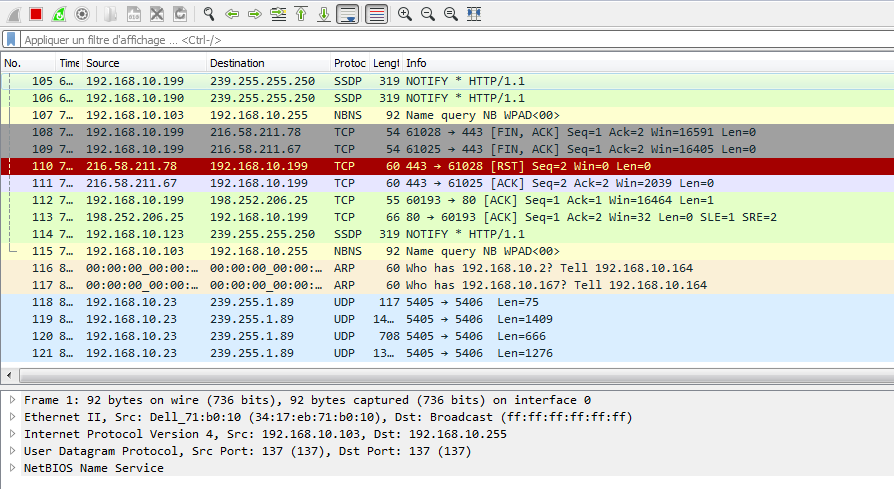
\includegraphics[width=12cm, height=8cm]{./images/wireshark.PNG}
\label{vueapprentissage}
\caption{Logiciel WireShark}
\end{figure}


L'image montre tous les packets qui transitent sur le réseau, cependant nous avons seulement besoin  de ceux qui sont liées au site. 

Il faut donc appliquer un filtre du type: 
 
\fbox{http.request \&\& not http.request.uri matches "(js|gif|png|jpg|css)\$" \&\& ip.dst == xx.xxx.xx.xxx}

\subsection{Note: xx.xxx.xx.xxx correspond à l'adresse Ip du site.}

Il ne reste plus qu'a exporter la capture en PDML depuis: \smallbreak
 Fichier > Exporter Analyse des paquets > As PDML XML
 
 \begin{figure}

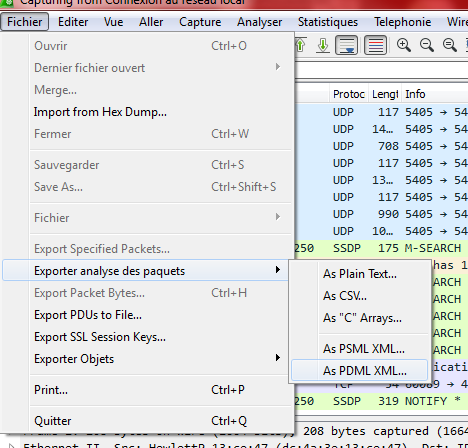
\includegraphics[width=5cm, height=6cm]{./images/exportpdml.png}
\label{iconevueapprentissage}
\caption{Icône pour exporter un fichier PDML}
\end{figure}
\newpage
\section{En ligne de commande}

Pour avoir la possibilité d'effectuer une capture en ligne de commande, vous devez avoir "Tshark" d'installé. \smallbreak
Dans le cas où celui-ci ne l'est pas,vous pouvez toujours l'installer avec la commande "apt-get install tshark"

\subsection{Note: Attention l'installation nécessite d'être en admin.}


Il existe 2 types de fichiers pour capturer les paquets qui transitent:
\begin{itemize}
\item .pdml
\item .pcap
\end{itemize}

Rocaweb prend seulement en charge les fichiers avec l'extension ".pdml".\smallbreak
Il est possible de traiter ces fichiers pour qu'ils aient cette extension. 
 
\begin{large}
sudo tshark -V -T pdml -r [PCAPSOURCE] -Y "http.request \&\& ip.src == [IPSOURCE] \&\& not http.request.uri matches \\ "(js|gif|png)\\\$\\ ""
\end{large}
 
\smallbreak
Vous pouvez également effectuer directement la capture réseau avec un fichier ayant l'extension ".pdml" avec la commande:  
 

\begin{large}
sudo tshark -V -T pdml -i eth0 -Y "http.request \&\& ip.dst == [IPDESTINATION] \&\& ip.src == [IPSOURCE] \&\& not http.request.uri matches \\ " (js|gif|png)\\ \$\\ "" > fichier-output.pdml

\end{large}











\chapter{La vue Data}
La vue "data" permet la visualisation des données. 

Le pré-requis pour la visualisation est d'avoir le fichier PDML du site.

La première étape consiste à importer le fichier PDML sur ROCAWEB. Le bloc "Sources" étant prévu à cet effet.

\begin{figure}
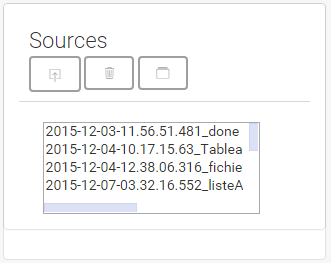
\includegraphics[width=8cm, height=6cm]{./images/blocdatasource.png}
\label{vueapprentissage}
\caption{Gestion des fichiers PDML}
\end{figure}

\begin{marginfigure}

\includegraphics[width=1cm, height=1cm]{./images/importpdml.png}
\label{iconevueapprentissage}
\caption{Icône pour importer un fichier PDML}
\end{marginfigure}

Pour importer le fichier PDML cliquer sur le bouton représenté en {\itshape figure 4} 



Vous pouvez ensuite parcourir vos dossiers pour aller chercher le fichier du type "xxx.pdml".

Votre fichier est maintenant présent dans votre liste. 

\subsection{Note: L'import peut être long, un message de confirmation vous indique la fin. Vous devez également recharger votre page pour que votre fichier s'affiche dans votre liste.}



Vous devez ensuite pré-traité vos fichiers. Il vous suffit de sélectionner le fichier que vous venez d'importer et de cliquer sur le bouton correspondant à la {\itshape figure 5}

\begin{marginfigure}

\includegraphics[width=1cm, height=1cm]{./images/pretraitementpdml.png}
\label{iconevueapprentissage}
\caption{Icône de pré-traitement de vos fichiers PDML}
\end{marginfigure}

\subsection{Note: Un message de confirmation vous indique la fin. Vous devez également recharger votre page pour que votre fichier s'affiche dans votre liste.}

Une fois votre fichier traité, celui-ci s'affiche dans la bloc "Pré-traitement" disponible en {\itshape figure 6}
\begin{figure}
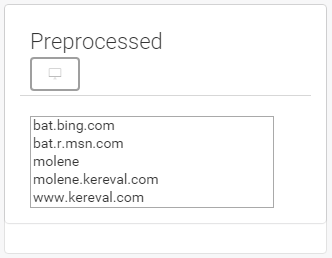
\includegraphics[width=8cm, height=8cm]{./images/blocpretraitement.png}
\label{iconevueapprentissage}
\caption{Gestion des pré-traitements}
\end{figure}


Vous pouvez visualiser l'arborescence de votre site en cliquant sur le bouton en {\itshape figure 7} 

\begin{marginfigure}

\includegraphics[width=1cm, height=1cm]{./images/visupretraitement.png}
\label{iconevueapprentissage}
\caption{Icône de visualisation de l'arbre}
\end{marginfigure}

Cela vous permet ainsi de visualiser l'arborescence de votre site.

\begin{figure}
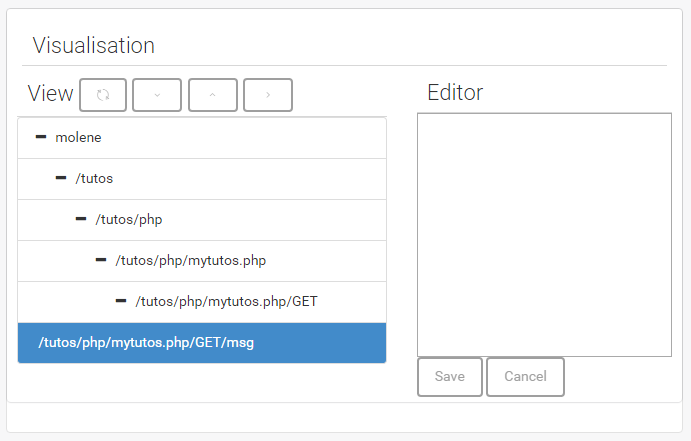
\includegraphics[width=11cm, height=11cm]{./images/arbosite.png}
\label{iconevueapprentissage}
\caption{Visualisation Arborescence du site}
\end{figure}


Vous pouvez dès à présent visualiser les données passé en paramètre dans les requêtes.
Il vous suffit de sélectionner un nœud et de cliquer sur le bouton présent en {\itshape figure 9}.

\begin{marginfigure}
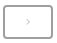
\includegraphics[width=1cm, height=1cm]{./images/visudonnees.png}
\label{iconevueapprentissage}
\caption{Icône de visualisation de l'arbre}
\end{marginfigure}

Les différentes données passées en paramètres lors de l'apprentissage du site  s'affichent dans l'éditeur({\itshape figure 8}).


\begin{figure}
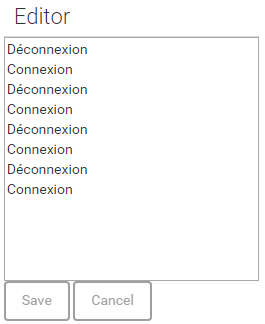
\includegraphics[width=8cm, height=7cm]{./images/editeurvisu.png}
\label{iconevueapprentissage}
\caption{Données passées en paramètre lors de la requête}
\end{figure}


\subsection{A savoir:}

\subsection{Dans le cas où les données vous paraissent incorrectes pour la génération des règles, vous pouvez modifier les données et cliquer sur le bouton "Save" ({\itshape figure 11}).}

\begin{marginfigure}

\includegraphics[width=1cm, height=1cm]{./images/savedonnees.png}
\label{iconevueapprentissage}
\caption{Icône de sauvegarde des données}
\end{marginfigure}

Maintenant que les données sont viables, vous pouvez accéder à la page "Learning" pour effectuer un apprentissage des règles (Chapitre Apprentissage). 

\chapter{Apprentissage}


Cette interface permet la génération des règles de sécurité.
 
Pour effectuer un apprentissage, vous retrouvez la partie pour le pré-traitement des données. 
 

\begin{marginfigure}

\includegraphics[width=1cm, height=1cm]{./images/visupretraitement.png}
\label{iconevueapprentissage}
\caption{Icône de visualisation de l'arbre}
\end{marginfigure}

Sélectionner le site sur lequel vous souhaitez effectuer un apprentissage et cliquer sur le bouton "Cluzterize" ({\itshape figure 12}). 



L'arborescence du site s'affiche dans le bloc "Visualisation". 
 
Enfin pour générer une règle de sécurité, sélectionner le site, le nœud, l'algorithme que vous souhaitez utiliser et cliquer sur le bouton "Run" ({\itshape figure 13}). 

\begin{marginfigure}
\label{iconevueapprentissage}
\caption{Vue apprentissage de règles}
\end{marginfigure}


\begin{figure}
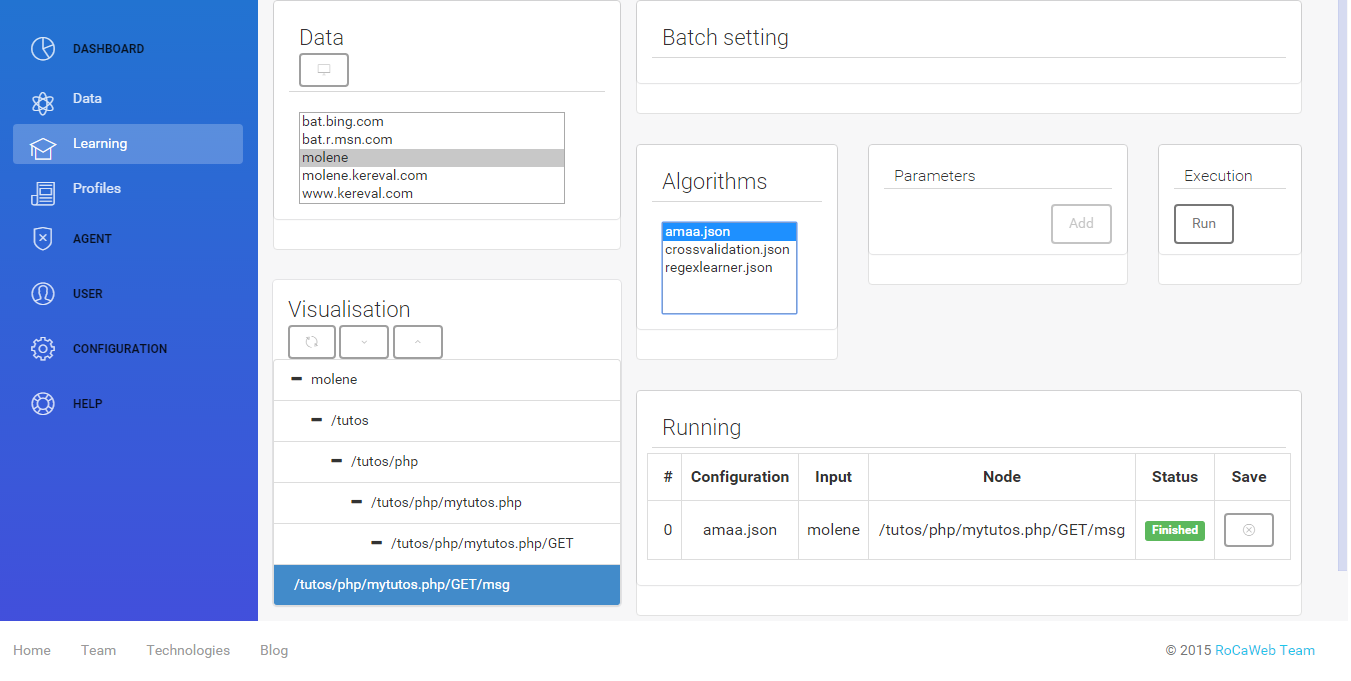
\includegraphics[width=15cm, height=12cm]{./images/learning.png}
\label{iconevueapprentissage}
\end{figure}
La configuration que vous avez sélectionné s'ajoute automatiquement dans le block "Running". Le statut de la configuration est modifié en fonction de son état d'avancement.  

\begin{itemize}
\item Finish
\item Running
\item Waiting
\end{itemize}

Dès que le statut est "Finish", vous avez accès à la règle depuis le menu Profiles

\section{Les nouveaux algorithmes}

\subsection{La longueur des attributs}
 \paragraph{Hypothèses}
  \begin{itemize}
   \item Les longueurs des valeurs du paramètre n'évoluent pas énormément entre les requêtes. 
   \item Exemple : certains champs d'un formulaire ou $token$ à taille fixe (identifiant de session) 
  \end{itemize}
 
 \paragraph{Cette évolution pouvant être représentée par une variable aléatoire $X$ ayant $\mu$ et $\sigma$ comme paramètres.}
 
 
 \paragraph{Théorème}
  Soit une variable aléatoire $X$ avec $Var[X] < +\infty$. Alors, pour tout $t > 0$, l'inégalité suivante tiens~\cite{mohri2012foundations} : 
    \begin{equation}
  p(|X - E[X]| \geq t \times \sigma_X) \leq \frac{1}{t^2}
 \end{equation}

 L'inégalité de Chebychev ne requiert que la connaissance de la moyenne et la variance. 
 L'inégalité de Chebychev lie la déviation d'une variable aléatoire de son espérance en terme de son écart type.

 
 
 \paragraph{Méthode de Chebychev appliquée à la longueur}
 \paragraph{Phase d'apprentissage}
  Soient : 
  \begin{itemize}
   \item $A$ un attribut d'une requête ;
   \item $A = \{a_i, i  = 1...n\}$ valeurs collectées et représentant un comportement sain. 
  \end{itemize}
   
   Déterminer: 
   \begin{itemize}
    \item $\mu$ : la moyenne des longueurs des $a_i$;
    \item $\sigma$ : la variance ;
   \end{itemize}

   
 



 \paragraph{Méthode de Chebychev appliquée à la longueur}

 \paragraph{Phase de détection}
 \label{detectional}
  Soient : 
  \begin{itemize}
  \item $a_k$ une valeur à évaluer;
   \item $\mu, \sigma$ : les valeurs déterminées précédemment. 
  \end{itemize}
   
 
 Variante :  
 \begin{equation}
  p(|X - \mu| > |l - \mu|) < p(l) = \left\lbrace \begin{array}{ll}
                                            \frac{\sigma^2}{(l-\mu)^2} & \textrm{Si l $\ge \mu$}  \\
                                            1 & \textrm{Sinon}
                                           \end{array}\right.
 \end{equation}

 $l$ est la longueur courante. Retourne $p(l)$

\paragraph{\textbf{Génération de règles pour AttributeLength}}
 
 Après l'apprentissage, la méthode génère $\mu$ et $\sigma$. Ces valeurs constituant le modèles sont stockées dans la collection $TX$ de ModSecurity\sidenote{\url{http://tiny.cc/saxt8x}}.
 Ces valeurs sont par la suite traité par le code Lua.
 
\begin{verbatim}
SecRule &ARGS:names "@ge 1" "setvar:TX.mean=mu,setvar:TX.std=sigma,chain,setvar:TX.name=names,..." 
SecRuleScript /opt/validation/attributelength.lua
 \end{verbatim}

Dans la règle SecRule, nous spécifions que lorsque que l'argument "manes'' de la collection ARGS est présent plus d'une fois, que ModSecurity doit enclencher la règle
et doit définir et affection au variable TX.mean=mean, TX.std=sigma, TX.threshold=seuil.

La règle SecRuleScript est chaînée à la précédent et aussi enclenché juste après la règle SecRuLe
Le script Lua, récupère alors les contenues de TX.mean, TX.std, TX.threshold et TX.name et effectue la validation décrite dans~\ref{detectional}. 
Si le script retourne une valeur différente de $nil$, ModeSecurity lève une alerte. 
 
 
\subsection{La distribution des caractères}

 \paragraph{Hypothèses}
  \begin{itemize}
   \item Les attributs ont une structure régulière;
   \item Les attributs peuvent être lues par des humains;
   \item Contiennent presque toujours des caractères imprimables;
%  \item Pour les binaires des critères peuvent aussi être déterminés. 
  \end{itemize}

  \paragraph{Phase d'apprentissage}
  \begin{itemize}
   \item Déterminer la distribution de référence ou ICD;
  \end{itemize}
  
  Soient :
   \begin{itemize}
    \item $A = \{a_1,a_2,...,a_n\}$;
    \item $E$ un alphabet; 
    \item $a_i$ sont définis sur $E^{*}$. 
   \end{itemize}
   Une distribution de caractères est définie par : 
  \begin{equation}
   CD = \{n_i, i=1..k\}
  \end{equation}




 \paragraph{Distribution de référence}
  \begin{itemize}
   \item Pour chaque paramètre déterminer le CD
   \item Trier décroissant CD
   \item $ICD = \{f_i = n_i/k, i=1...k\}$
   \item Pour $k=256$, tous les caractères possibles. 
  \end{itemize}



 \paragraph{Phase de détection}
  Soient :
  \begin{itemize}
   \item le CD d'une valeur d'un paramètre
   \item et l'ICD de toutes les valeurs observées
  \end{itemize}
   Déterminer la probabilité en utilisant un test de $\chi^2$
 





 \paragraph{Test de  $\chi^2$}
  $\left\lbrace\begin{array}{ll}
    H_0&\textrm{: La distribution de caractères provient de l'ICD} \\
    H_1 &\textrm{: La distribution ne provient pas de l'ICD.}
   \end{array}\right.
    $

  \begin{enumerate}
   \item  Fixer le nombre de ''bins``.
    Six ''bins`` : $0, 1-3, 4-6, 7-11, 12-15, 16-255$
   \item Calculer : \begin{equation}
                     \chi^2 = \sum_{i=1}\frac{(O_i-E_i)^2}{E_i}
                    \end{equation}
     Où : 
     \begin{itemize}
      \item $O_i$ les valeurs observés;
      \item $E_i$ = $f_i\times length(a_k)$ . 
     \end{itemize}
   
   \item Retourner la $p-value$, en fonction du nombre de degrés de liberté.
  \end{enumerate}
 

\paragraph{\textbf{Génération de règles pour la distribution des caractères (ACD)}}

\begin{verbatim}
SecRule &ARGS:names "@ge 1" "setvar:TX.icd0=0.16,setvar:TX.icd1=0.32,setvar:TX.icd2=0.18,\\
setvar:TX.icd3=0.16,setvar:TX.icd4=0.07,setvar:TX.icd5=0.08,..." 
SecRuleScript /opt/validation/attributecharacterdistribution.lua
\end{verbatim}

Le format de règles est similaire à celui que nous avons décrit précédemment pour la longueur des paramètres. 
Cette fois-ci la validation se fait par un autre script qui récupère les TX.icd0 à TX.icd5. 

\paragraph{\textbf{Remarque}}
L'ACD ne génère pas de règles lorsque, les données ne sont pas assez ''riches``. C'est à dire l'alphabet doit contenir plus de 17 caractères différents. 

\chapter{Les profiles}

La vue profil permet la visualisation des profils et de leurs modifications.
 
Pour y accéder, cliquer sur "Profiles" depuis le menu.
 
La page est constitué d'un bloc "Profiles", d'un bloc "Visualisation", et d'un bloc "Management".
 
Chaque configuration avec le statut "Finish" est présente dans le bloc "Profiles" ({\itshape figure 14}). 

\begin{figure}
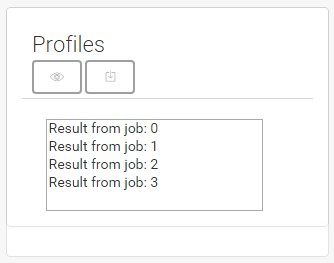
\includegraphics[width=8cm, height=7cm]{./images/profilevisu.png}
\label{iconevueapprentissage}
\caption{Données passées en paramètre lors de la requête}
\end{figure}

Lorsque vous sélectionnez un résultat d'apprentissage dans la liste. et que vous cliquer sur le bouton représenté en {\itshape figure 15}, cela affiche l'arbre sur lequel la règle a été généré. 

\begin{marginfigure}

\includegraphics[width=1cm, height=1cm]{./images/visuresultjobs.png}
\label{iconevueapprentissage}
\caption{Icône permettant l'affichage de l'arbre}
\end{marginfigure}

 
Le second bouton ({\itshape figure 16}), permet le téléchargement d'un fichier avec l'extension ".txt". Ce fichier s'ouvre avec n'importe quel éditeur de texte et contient la règle de sécurité généré précédemment.  

\begin{marginfigure}

\includegraphics[width=1cm, height=1cm]{./images/visudownjobs.png}
\label{iconevueapprentissage}
\caption{Icône permettant le téléchargement de la règle de sécurité}
\end{marginfigure}

\section{Déploiement des règles}
Un VM d'exemple est fournie pour tester Rocaweb.
La VM est une distribution Ubuntu configuré avec Apache et Modsecurity

Une fois un profile généré, renommer le fichier en fichier .conf

Placer le fichier générer sur la VM par exemple dans le dossier : /etc/modsecurity/sut\_rules/

La configuration de reverse proxy est précisée dans le fichier : /etc/apache2/sites-enabled/reverse.conf

La référence des fichiers de règles modsecurity est précisé par la ligne de configuration :Include "/etc/modsecurity/sut\_rules/*.conf"

La configuration du reverse proxy à été faite à titre d'exemple sur un site en interne, elle doit être modifiée pour référencer le site testé.

\begin{verbatim}

ProxyPass /tutos http://192.168.10.76/tutos
<Location /tutos/>
ProxyPassReverse /tutos/
SetOutputFilter INFLATE;proxy-html;DEFLATE
ProxyHTMLURLMap /tutos/ /tutos/
ProxyHTMLURLMap / /tutos/
ProxyHTMLURLMap http://192.168.10.76/tutos http://192.168.10.101:8086/tutos
RequestHeader unset Accept-Encoding
</Location>

\end{verbatim}


% \chapter{Les algorithmes d'apprentissage}

\chapter{Conclusions}
Nous allons maintenant aborder les cas où, le programme que vous aller utiliser rencontre des problèmes :  
\begin{itemize}
\item Le traitements des PDML peut lever des Exceptions 

\item Lorsque vous ne choisissez par un fichier pour l'apprentissage ou un algorithmes

\item Des restrictions liés au systèmes d'exploitation. Vous n'avez pas besoin de droit \textbf{root} pour utiliser ce programme, mais nous avons mis en œuvre deux processus légers qui surveillent
les dossiers ''/resource/learningdata`` et ''profiles`` pour qu'en cas de modifications les vues associés soient automatiquement mis à jour. Or dans certain cas des exceptions ont été levées. 

\item L'adaptation automatique des vues par rapport aux différents navigateurs, ainsi que l'adaptation des taille des écrans est en cours d'amélioration. 

\item Nous n'avons pas encore intégré une validation des entrées utilisateur. Ce qui veut dire que vous êtes libres de tester des injections de toutes sortes dans les champs recevant les paramètres. Normalement, vous devez voir des exceptions. Normalement...

\end{itemize}

Nous concluons sur le fait que la recherche et le développement sont toujours en cours. Il existe des problèmes connus, ils seront solutionnés dans les versions futures.
Nous allons mettre en place des outils de mises à jours automatique et de réception des bugs et des souhaits. 


\end{document}          
